\chapter{Context of the work}
\phantomsection


\setcounter{secnumdepth}{0} % Set the section counter to 0 so next section is not counted in toc
% ----------------------- Introduction ----------------------- %
\section{Introduction}
This chapter introduces the general context of this report.
We start by presenting the frame of the project as well as the host company.
Then comes the enumeration of the problems which led to the realization of the project.
We wrap it up by defining the methodology we’ve followed to carry out our work.

\setcounter{secnumdepth}{2} % Resume counting the sections for the toc with a depth of 2 (Sections and sub-sections)
% ----------------------- General framework of the internship ----------------------- %
\section{General framework of the internship}
This project was carried out within the frame of obtaining a bachelor’s degree in Computer Science at the Higher Institute of Informatics and Mathematics of Monastir (ISIMM).
The internship took place fully remotely at Incedo Services GmbH for five months starting from the 15th of January 2024 to the 15th of June 2024 with the purpose of further developing an existing software solution of the company as well as working on a new feature, which is the reward system.

% ----------------------- Company overview ----------------------- %
\section{Company overview}
This section introduces the host company {\bf Incedo Services GmbH} as well as the services it offers.
\subsection{About Incedo}
"We are a young software development and consulting firm located in Stuttgart.
We help our clients to develop exciting digital products and solutions and we also love to bring our own ideas into life from time to time." \cite{about-incedo}
\begin{figure}[H]
    \centering
    \makebox[\textwidth]{
\includegraphics[width=12cm]{src/assets/images/incedo-logo_bg-trans-white_rgb.png}}
    \caption{Logo of Incedo Services GmbH}
    \label{fig:logo-of-incedo}
\end{figure}

% ----------------------- Stating the problem ----------------------- %
\section{About Aermax}

The company Aermax, created by Max Wörner, is located in Stuttgart Germany, and is associated with industrial alpinism. They offer professionals working with high-altitude or deep-location works by use of industrial alpinism techniques. An industrial alpine climber is a specialist trained in work at great heights or depths. During operations, the work of industrial climbers is carried out using a methodology known as a rope access technique. This technique enables the craftsmen to execute their works in a very difficult location without using scaffolding or lifts.


\subsection*{Key Advantages of Industrial Climbers}
\begin{itemize}
  \item Capacity to work on any height or depth
  \item With the use of ropes, a flexible way of deployment
  \item Execution of work without scaffolding and lifts
  \item Cost-effective and efficient
  \item Operational without interrupting business or production processes
  \item Less preparation time
  \item Capability of short-notice emergency deployment
\end{itemize}

With these advantages, Aermax secures that their services are effective, adaptive, and flexible with any surrounding environment, which is quite challenging, while maintaining a higher level of safety and efficiency.

\begin{figure}[H]
    \centering
    \makebox[\textwidth]{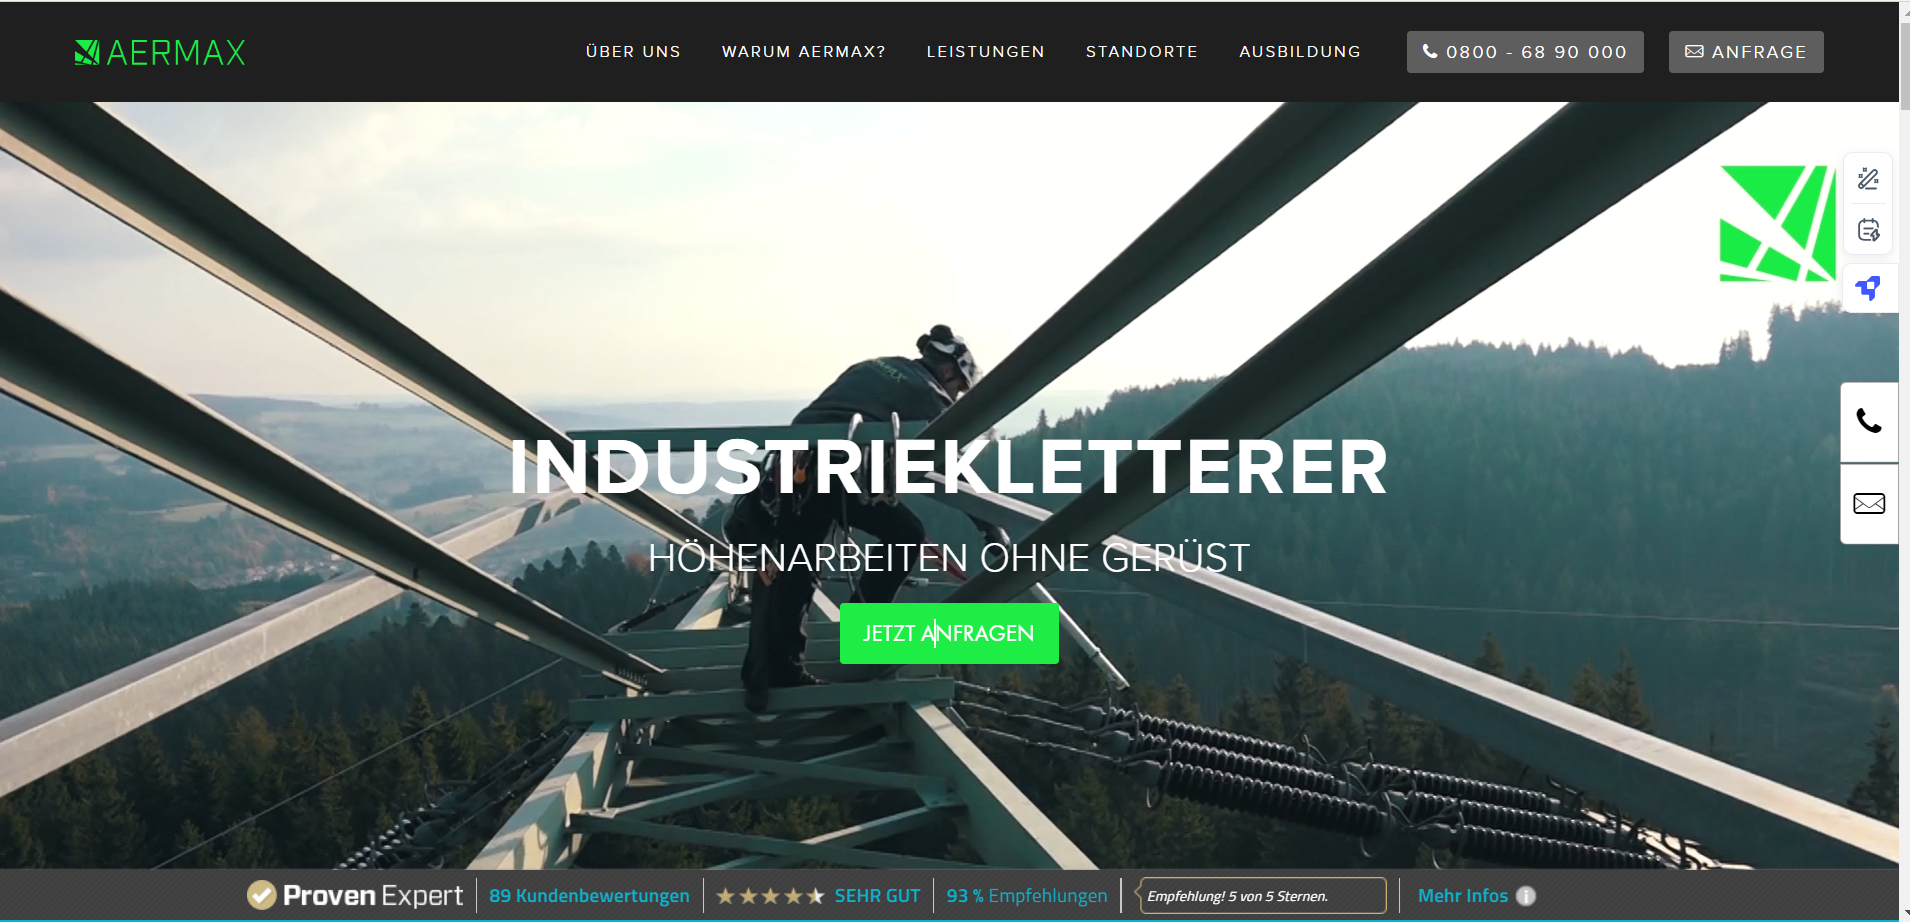
\includegraphics[width=12cm]{src/assets/images/aermax.PNG}}
    \caption{Aermax’s website}
    \label{fig:aermax-website}
\end{figure}

The client wanted to develop a platform to manage all their work, especially between employees-and-subcontractors, better known as externs.

\section{Competitor Benchmarking}
This section will discuss the analysis of the Aermax platform: review of the features, capabilities, and performance. The goal is to see the strong and weak sides of this service and compare it to industry standards. This analysis can act as a guideline on how to improve our platform to effectively manage high-altitude projects.
\subsection{Competitors Selection}
In the current solutions study, we have evaluated various platforms and chosen two which most closely fit our needs. We will give an overview of the chosen solutions and the main features and functionalities thereof.

\subsection{Blauarbeit}
Blauarbeit is an online marketplace where German citizens can look for experts to help them with hard and sometimes dangerous tasks.
It's like a big directory filled with experts who are good at fixing effects like broken pipes, or erecting new structures.
That way, a person can easily find the right fit for the job instead of searching everywhere. Moreover, Blauarbeit assures that workers are reliable and secure whether it is fixing a dense roof or cleaning at a high altitude and dangerous place.


\begin{figure}[H]
    \centering
    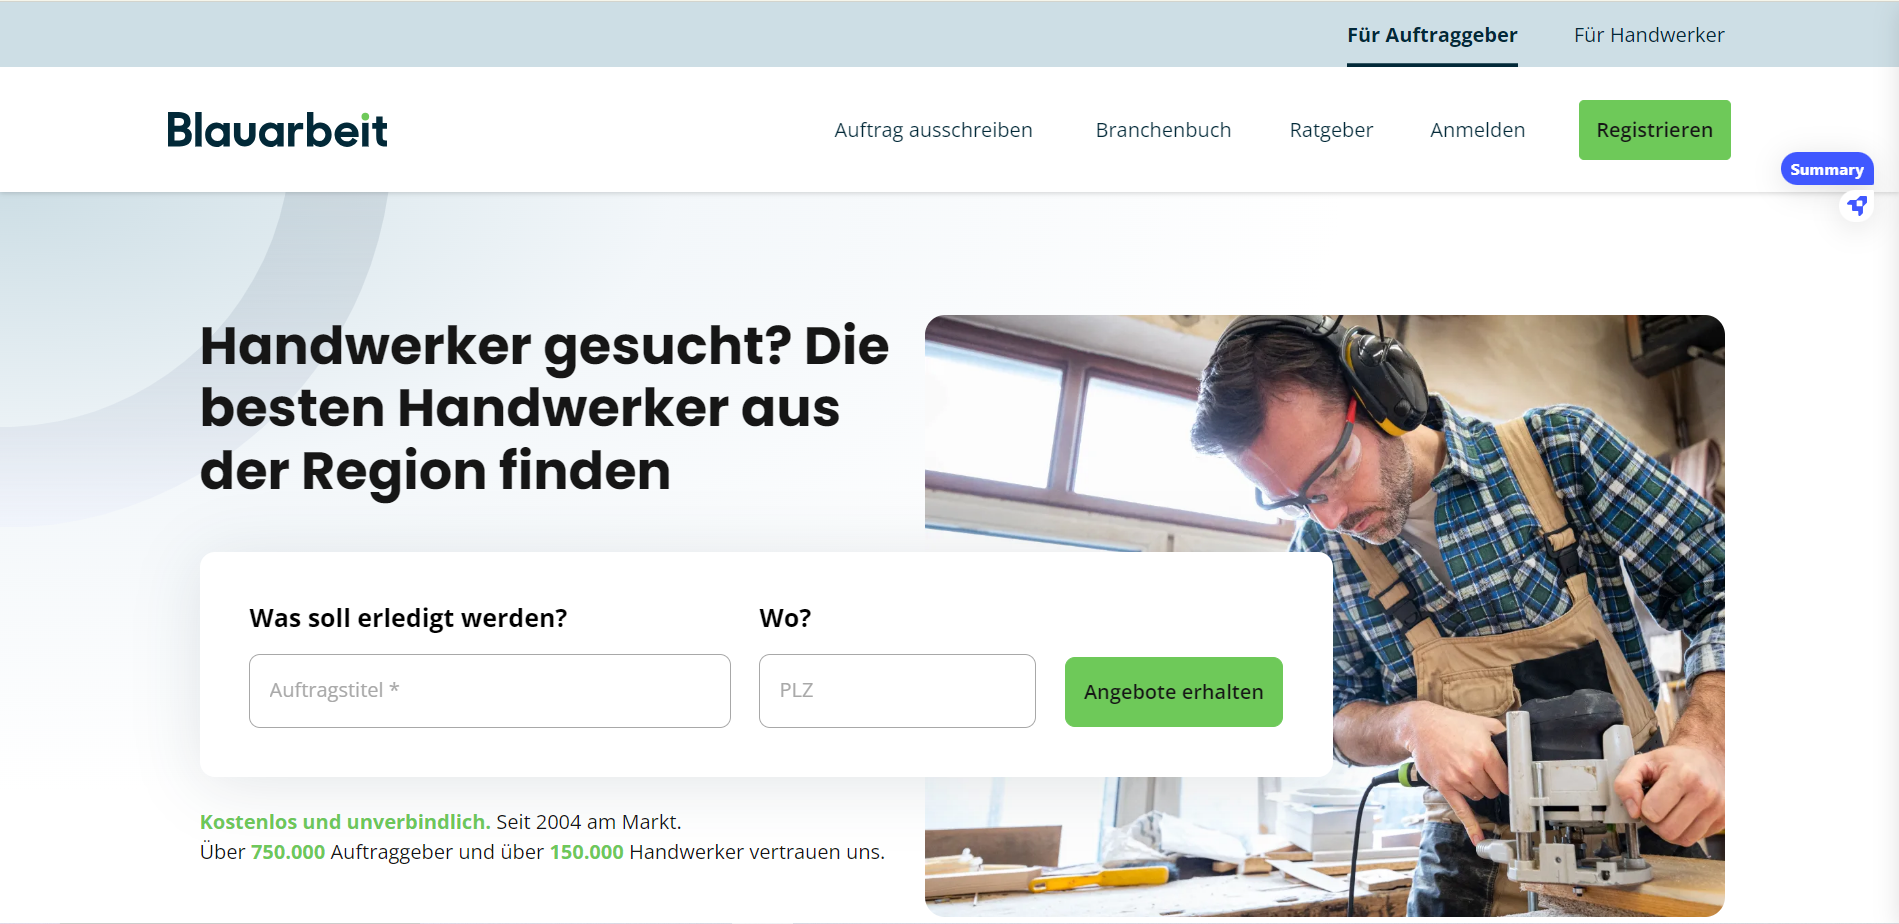
\includegraphics[width=\linewidth]{src/assets/chapters/Blaurabeit.PNG}
    \caption{Blaurabeit Homepage}
    \label{fig:blaurabeit_image}
\end{figure}


\subsection{MyHammer}
MyHammer is a German online portal that offers homeowners and businesses the option to find local craftsmen and service providers for a wide variety of construction,and repair work.
MyHammer offers a set of features such as a huge variety of services provided, transparent bidding, and a mobile-friendly interface.


\begin{figure}[H]
    \centering
    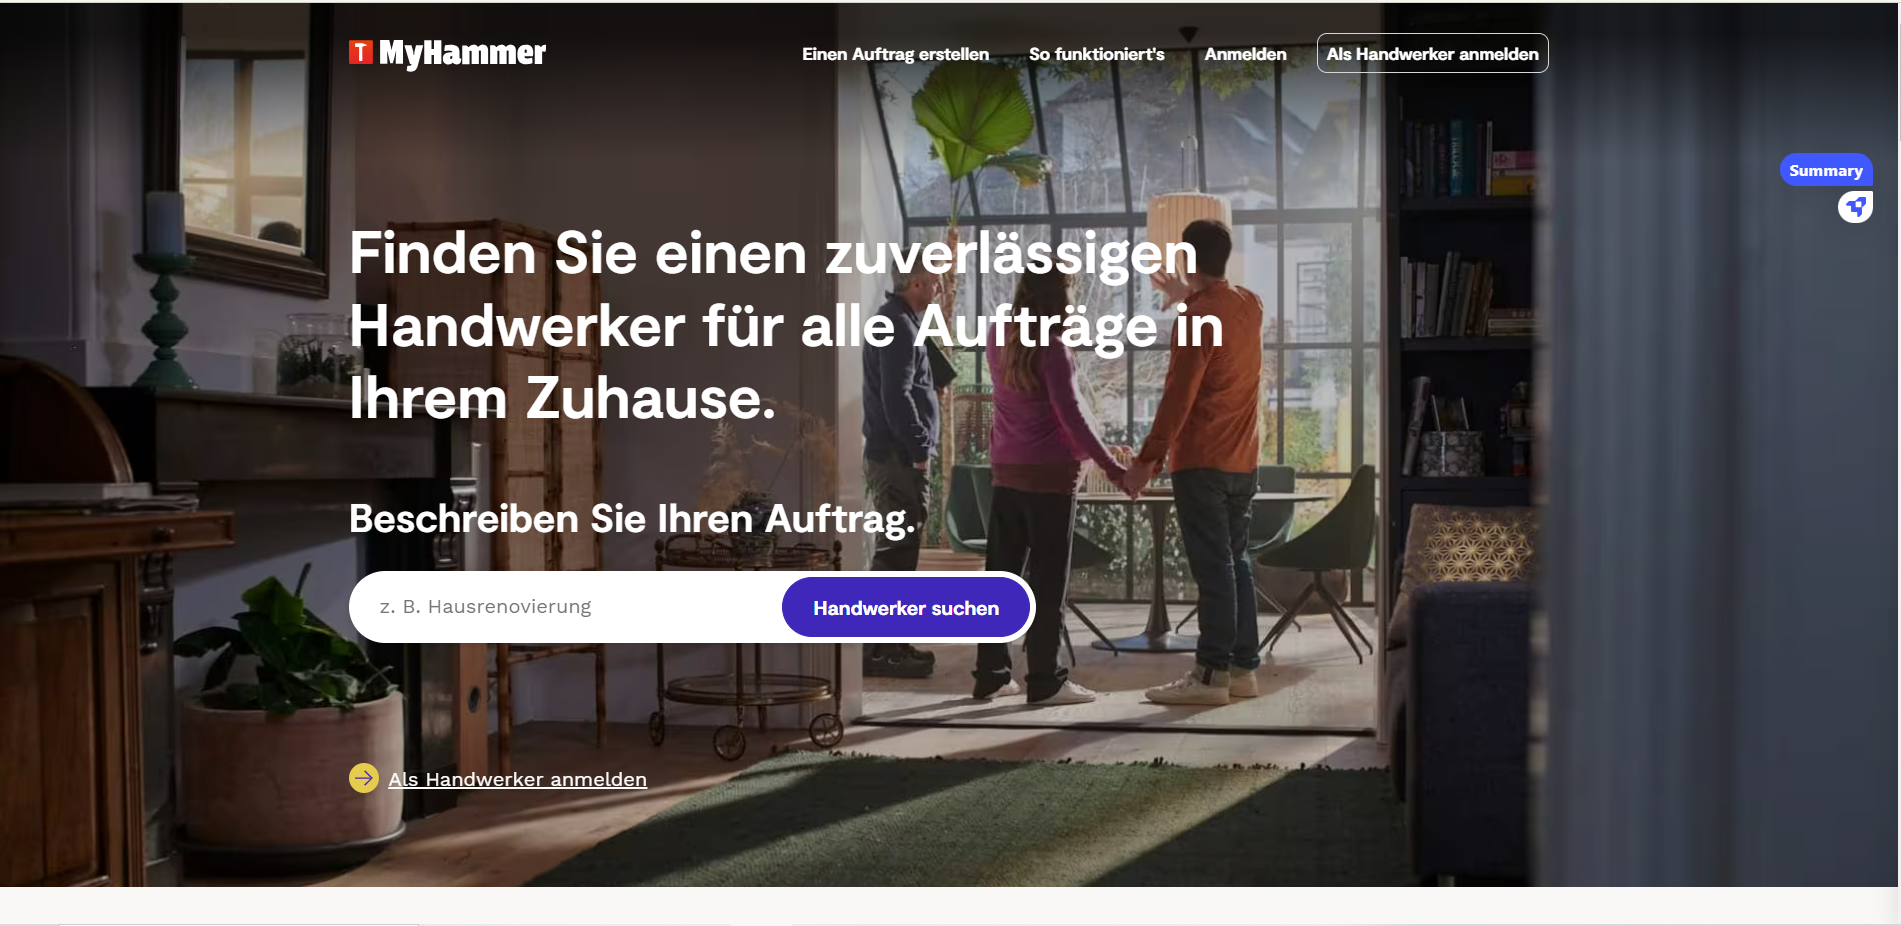
\includegraphics[width=\linewidth]{src/assets/chapters/myHammer.PNG}
    \caption{MyHammer Homepage}
    \label{fig:myhammer_image}
\end{figure}



\subsection{Aermax}
Aermax is a company that specializes in the provision of services at altitudes. It specializes in works that require preciseness and safety and expertise. One of the aspects of the works involves the provision of services that make buildings last and remain viable for a long time. 


\begin{figure}[H]
    \centering
    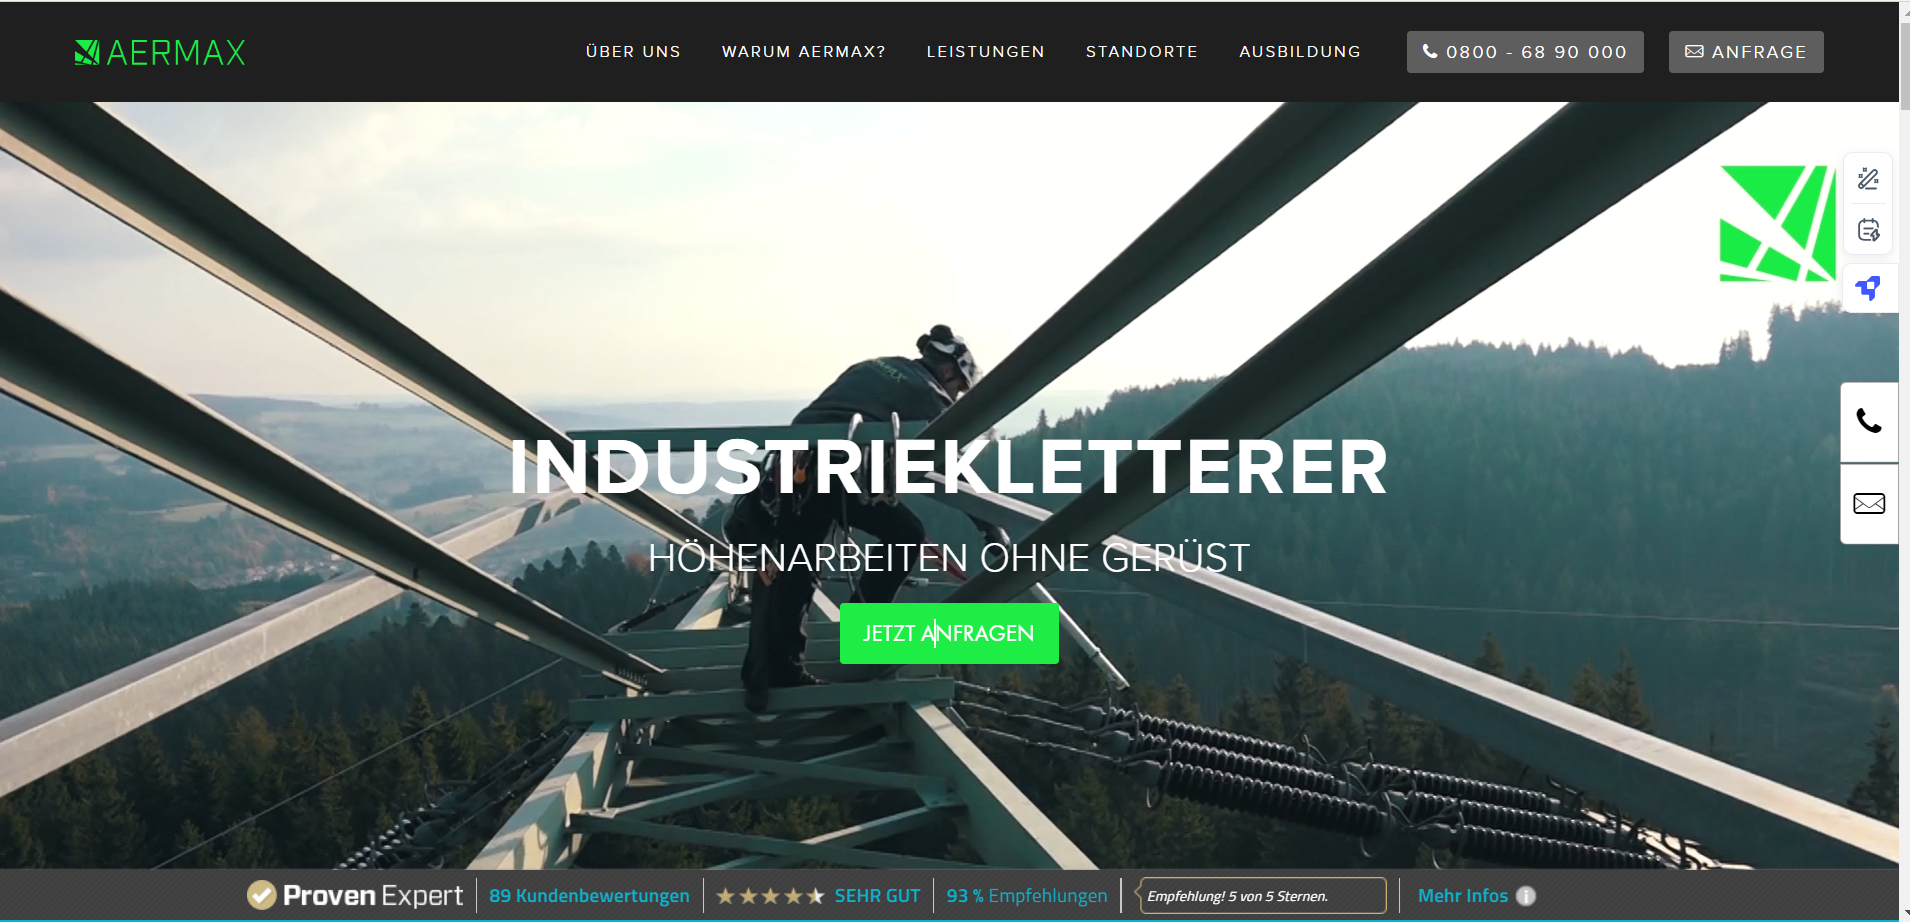
\includegraphics[width=\linewidth]{src/assets/images/aermax.PNG}
    \caption{Aermax Homepage}
    \label{fig:aermax_image}
\end{figure}

\subsection{Competitors Selection}
We are conducting a thorough assessment of project management platforms for industrial climbers to improve user experience and streamline operational processes. We will evaluate their functionalities, strengths, and weaknesses against 7 key criteria tailored to our project's needs and select the platform that best fits our requirements.

\begin{itemize}
    \item \textbf{C1: User Interface:} How the platform is designed regarding the interface and navigation of the platform to create a good experience for both technicians and project managers.

    \item \textbf{C2: Task Management:} How efficient is the platform in managing projects, including task assignment, progress tracking, and deadline setting.

    \item \textbf{C3: Document Management:} How the platform manages project documents, user files, the daily reports and performance’s reports.
    \item \textbf{C4: Communication Tools:} How far the platform supports communication between project managers, worker, and customers including real-time messaging, notifications.

    \item \textbf{C5: Safety Compliance:} How the platform can ensure compliance with safety regulations and standards that pertain to industrial climbing projects, tracking certifications, training records, and safety procedures.
    \item \textbf{C6: Equipment Management:} How the platform manege equipment used for industrial climbing projects.
    \item \textbf{C7: Project Planning and Scheduling:} How efficient the platform is in project planning and scheduling features, and timeline management.
\end{itemize}

\begin{longtable}{|p{2cm}|p{3.5cm}|p{3.5cm}|p{3.5cm}|}
    % Table header information for the first part
    \caption{Comparison of Project Management Platforms for Industrial Climbers} \\
    \hline
    \textbf{Criteria} & \textbf{MyHammer} & \textbf{Blauarbeit} & \textbf{Aermax}  \\
    \hline
    \endfirsthead
    
    % Table continuation header information
    \hline
    \textbf{Criteria} & \textbf{MyHammer} & \textbf{Blauarbeit} & \textbf{Aermax}  \\
    \hline
    \endhead
    
    % Footer at the end of each page (if needed)
    \hline
     
    
    % Footer at the end of the table (if needed)
    \hline
    \endlastfoot
    
    % Table content for Part 1
    C1: User Interface &  User-friendly interface for homeowners and service providers to connect for  projects.& Straightforward interface for customers and service providers to post and bid on household service tasks. & Easy-to-use design for admins, workers, and customers. The UI lacks a lot of refinments. \\ 
    \hline
    C2: Task Management & Lack of a dedicated task management features for organizing and tracking project progress. &  Lack of a dedicated task management features.Blauarbeit  does not offer tools specifically for task management within projects. & Essential task management features for project organizing and tracking progress is what Aermax provides. \\
    \hline
    C3: Document Management & Lack of a dedicated document management features. & Lack of a dedicated document management features. & Aermax provide a whole separe service to document management
    \\
    \hline
    
    % Table content for Part 2, continues in the same longtable environment
    C4: Communication Tools & A basic communication tool for homeowners and service providers to discuss project details and negotiate terms. & A standard communication tool for customers and service providers to negotiate job requirements and arrangements. & A standard chat channel for admins and workers, to discuss project progress and details. \\
    \hline
    C5: Safety Compliance & No specific safety compliance features for home improvement projects. & No dedicated safety compliance features for household services. & Lack of safety compliance features for construction and climbing services. \\
    \hline
    C6: Equipment Management & A fully integrated equipment management tool, to automate tracking and  management of equipment assets that can be used to complete projects efficiently. & An automated equipment management feature, providing scalable solutions for tracking and managing equipment assets across projects. & A simple and standard equipment management feature which isn’t maintainable and extensible.\\
    \hline
    C7: Project Planning and Scheduling & Lack of specific project planning or scheduling tools. & Lack of specific project planning or scheduling tools. & An efficient tool for managing and planning projects. \\
    \hline
\end{longtable}

% ----------------------- Assessment of the case ----------------------- %
\section{Assessment of the case}
This chapter shall evaluate the current state of the project, its strengths and weaknesses, propose solutions for its issues, and outline its implementation steps. The systematic approach is aimed at enhancing the performance of the project and user satisfaction.

\subsection{Describing the work procedure}
The work on any project, first of all, needs to be preceded by the profound study of the existing ones, undermining the strengths and weaknesses of the current system, and business decisions which should be taken into account during the conception and realization.

\subsection{Criticizing the current state}
After studying the existing, we can determine its limitations:

\subsubsection{Functional Issues}
\begin{itemize}
    \item Functionalities are not working as expected.
    \item New features are yet to be developed.
    \item Parts of the application need complete overhauling to meet the client's requirements.
\end{itemize}


\subsubsection{Technical Issues}
\begin{itemize}
    \item Since cron jobs are running for the whole day, bugs are hard to respond to fast enough because we can only deploy once at the end of the day.
    \item Many bugs remain unfixed.
    \item The code needs refactoring due to some bad practices that make the app take more time to execute.
\end{itemize}

\subsection{Proposed solution}
With the problems identified, we make the following proposals for the way forward.

\begin{itemize}
    \item First, existing features will be enhanced to ensure that they work as they should. This will entail a keen review and subsequent test of the features to identify and fix any bugs.
    \item In addition, new features will be developed based on priority to ensure that the application meets all of the client's requirements.
    \item There will also be thorough refactoring of the codebase to remove bad practices and optimize performance.
    \item The UI/UX is also recommended to be enhanced for a better user experience. The proposed solutions should be aimed at greatly enhancing the general performance of the application, reliability, and user satisfaction.
    \item Build a new feature: Reward System to make Aermax's users more engaged and motivated.
\end{itemize}

\begin{figure}[H]
    \centering
    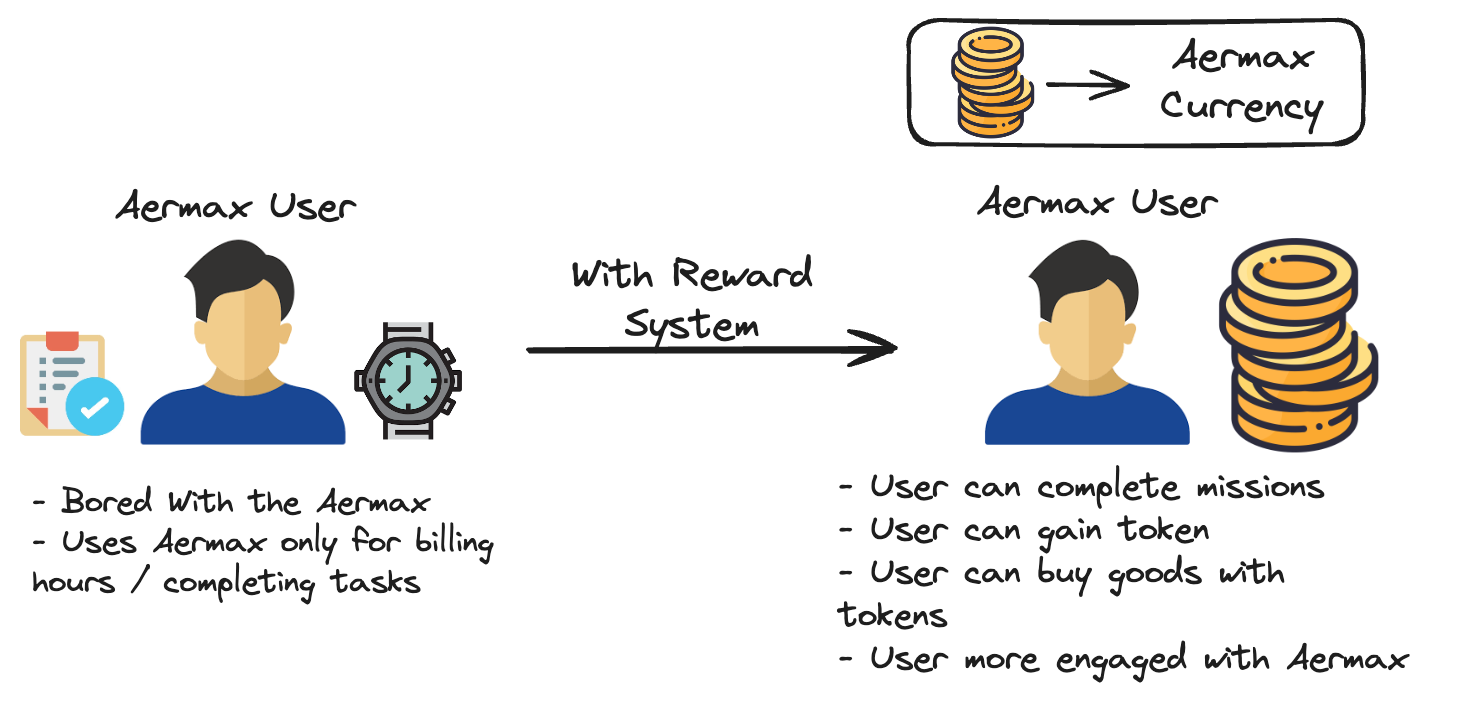
\includegraphics[width=0.7\textwidth]{src/assets/diagrams/rewardexplain.png}
    \caption{Reward System Overall View}
    \label{fig:Reward_System_explain_image}
\end{figure}

\begin{figure}[H]
    \centering
    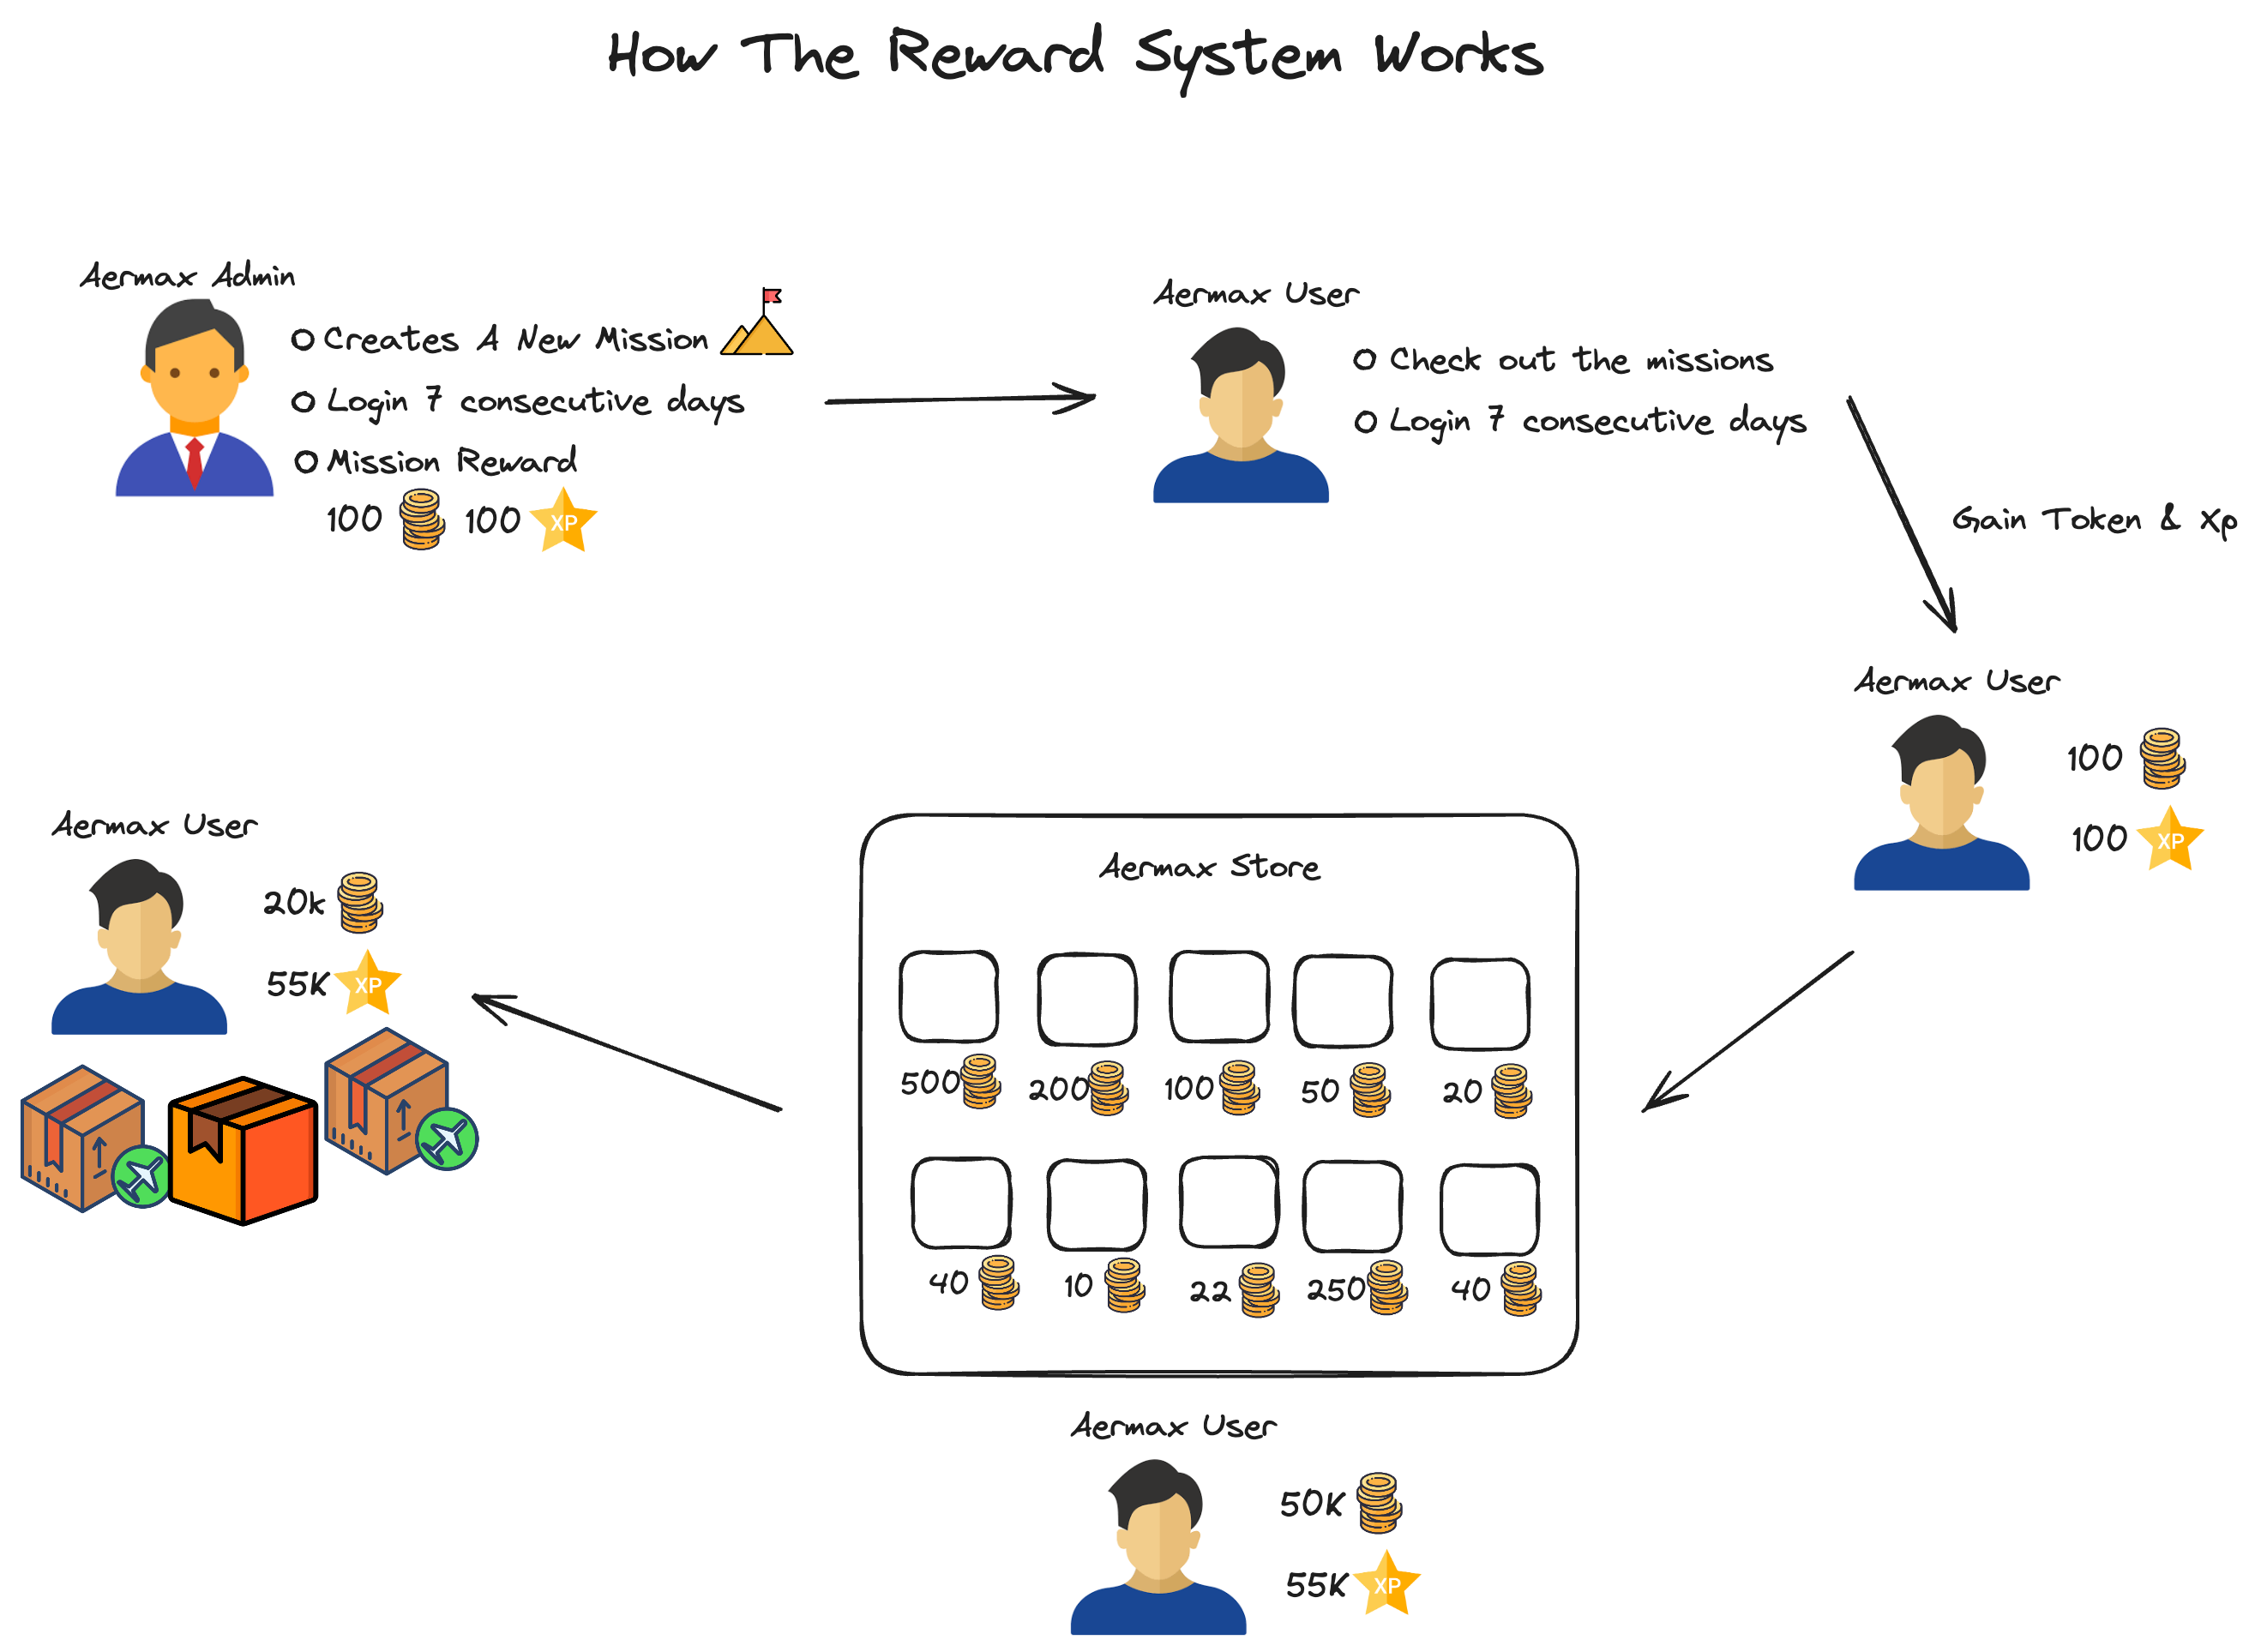
\includegraphics[width=1\textwidth]{src/assets/diagrams/rewardexplain2.png}
    \caption{Reward System Detailed Scenario}
    \label{fig:Reward_System_detailed_explain_image}
\end{figure}
   

\subsection{Work to Be Done}
\begin{itemize}
    \item Develop the major feature: the reward system.
    \item  Deploy the reward system into staging and then production.
    \item Enhance existing features to ensure they work as expected.
    \item Conduct a thorough review and testing of functionalities to identify and fix any bugs.
    \item Develop new features to meet the client's requirements.
    \item Refactor the codebase to eliminate bad practices and improve performance.
    \item Improve the UI/UX design to enhance user experience and satisfaction.
\end{itemize}

% ----------------------- Development Methodology ----------------------- %
\section{Development Methodology}
\subsection{Agile methodology}
Agile is a structured and iterative approach to project management and product development.
It recognizes the volatility of product development, and provides a methodology for self-organizing teams to respond to change without going off the rails.

\subsection{Scrum methodology}
The Scrum team commits to the completion of an increment of work, which is potentially shippable, through set periods of time called sprints.
They strive to build a learning loop in order to quickly collect and integrate customer feedback.
Scrum teams embrace specific roles, create special artifacts, and hold regular ceremonies to keep things moving.


\begin{figure}[H]
    \centering
    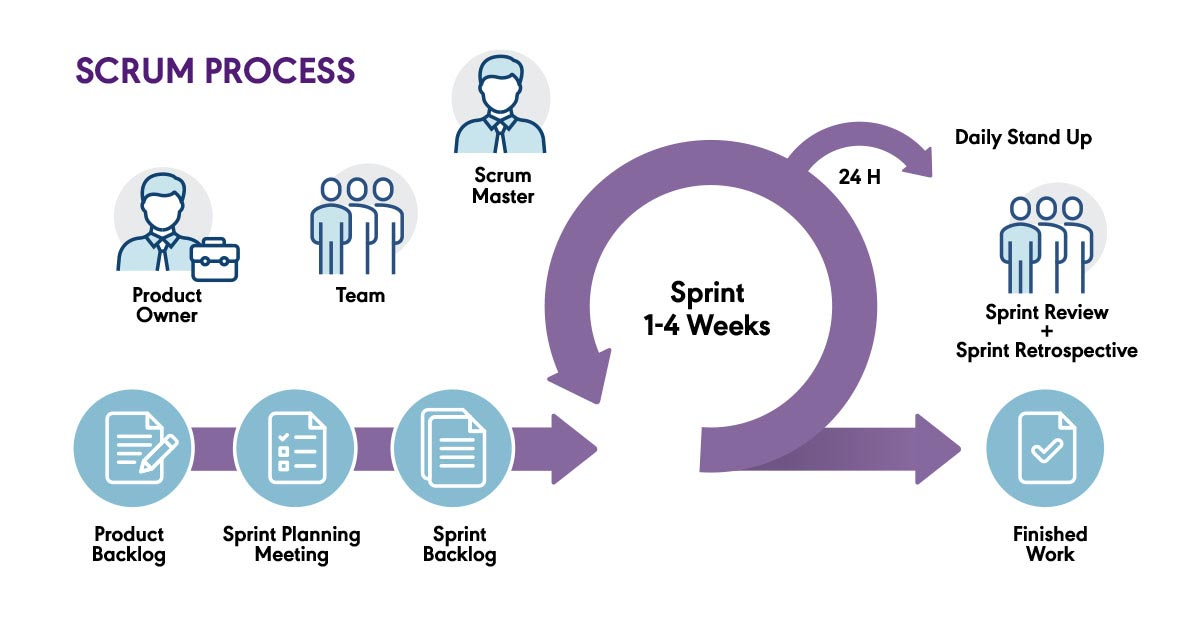
\includegraphics[width=0.7\textwidth]{src/assets/chapters/blog-scrum-process-opt.jpg}
    \caption{The Scrum Framework}
    \label{fig:Scrum_Framework_image}
\end{figure}


\subsection{Kanban methodology}
Kanban is all about visualizing your work, limiting work in progress, and maximizing efficiency (or flow).
Kanban teams focus on reducing the time a project takes from start by using a Kanban board to continuously improve their flow of work.
To explain more in details, Kanban is based on a continuous workflow structure that keeps teams nimble and ready to adapt to changing priorities.
Work items —represented by cards— are organized on the board where they flow from one stage of the workflow or column to the next.
Common workflow stages are To Do, In Progress, In Review, and Done.

\subsection{Scrumban methodology}
ScrumBan is a hybrid Agile methodology that combines elements of Scrum and Kanban. Here are some important points about Scrumban:

\begin{itemize}
    \item Hybrid Methodology: ScrumBan merges the flexibility of Kanban with the structure of Scrum to optimize workflow.
    \item Continuous Improvement: Similar to Kanban, Scrumban focuses on continuous improvement with the visualization of workflow and by limiting Work in Progress (WIP).
    \item Iterative Approach: Scrumban retains the iterative approach of Scrum—allowing periodic review and adaptation of processes.
    \item Adaptive Planning: A team can plan in a way that it can change the priorities and resources, if so required, as per the changing requirements while using Scrumban.
    \item Lean Principles: Scrumban adopts the principles of Lean—like waste elimination and maximization of value delivery—to streamline processes.
\end{itemize}

\begin{figure}[H]
    \centering
    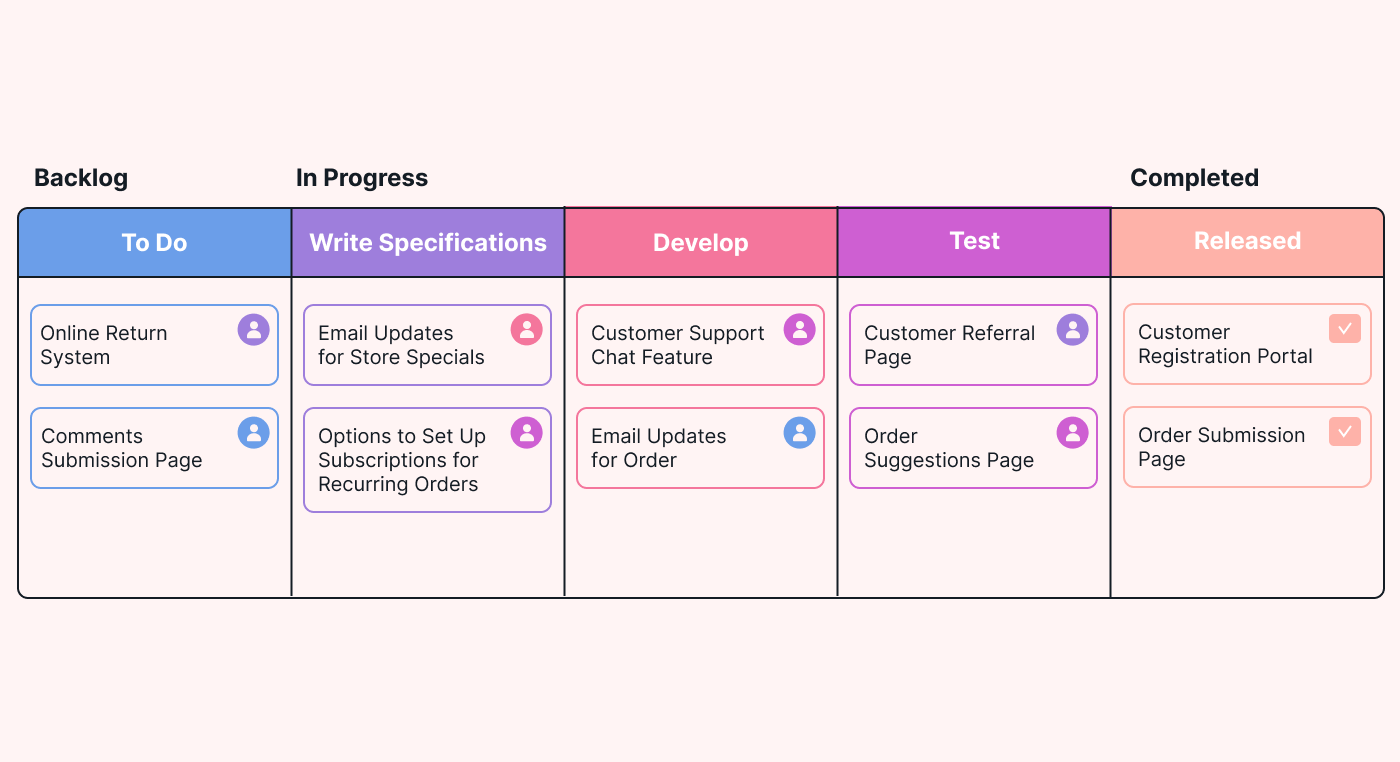
\includegraphics[width=0.7\textwidth]{src/assets/chapters/Scrumban.png}
    \caption{The Scrumban board}
    \label{fig:Scrumban_image}
\end{figure}

\newpage
\subsection{The choice for AERMAX}
Scrumban has been chosen as the preferred development methodology for the following reasons:
\begin{itemize}
    \item \textbf{Flexibility:} ScrumBan is a very flexible approach that brings some structure to Scrum while maintaining a high level of adaptability, similar to Kanban, which includes fast responses to changing priorities while maintaining a framing order for work.
    \item \textbf{Continuous Improvement:} Scrumban encourages continuous improvement, and teams can evolve their process over time.
    \item \textbf{Reduced Waste:} Scrumban introduces the principle of just-in-time delivery of user stories and WIP limits to ensure minimization of wastes.
    \item \textbf{Improved Visibility:} Visual boards improve the visibility of work, enabling transparency and encouraging collaboration.
    \item \textbf{Optimized Flow:} Scrumban is a way of optimizing flow by balancing Kanban flexibility with structured Scrum, enabling teams to build value consistently and predictably.
\end{itemize}

\begin{figure}[H]
    \centering
    \makebox[\textwidth]{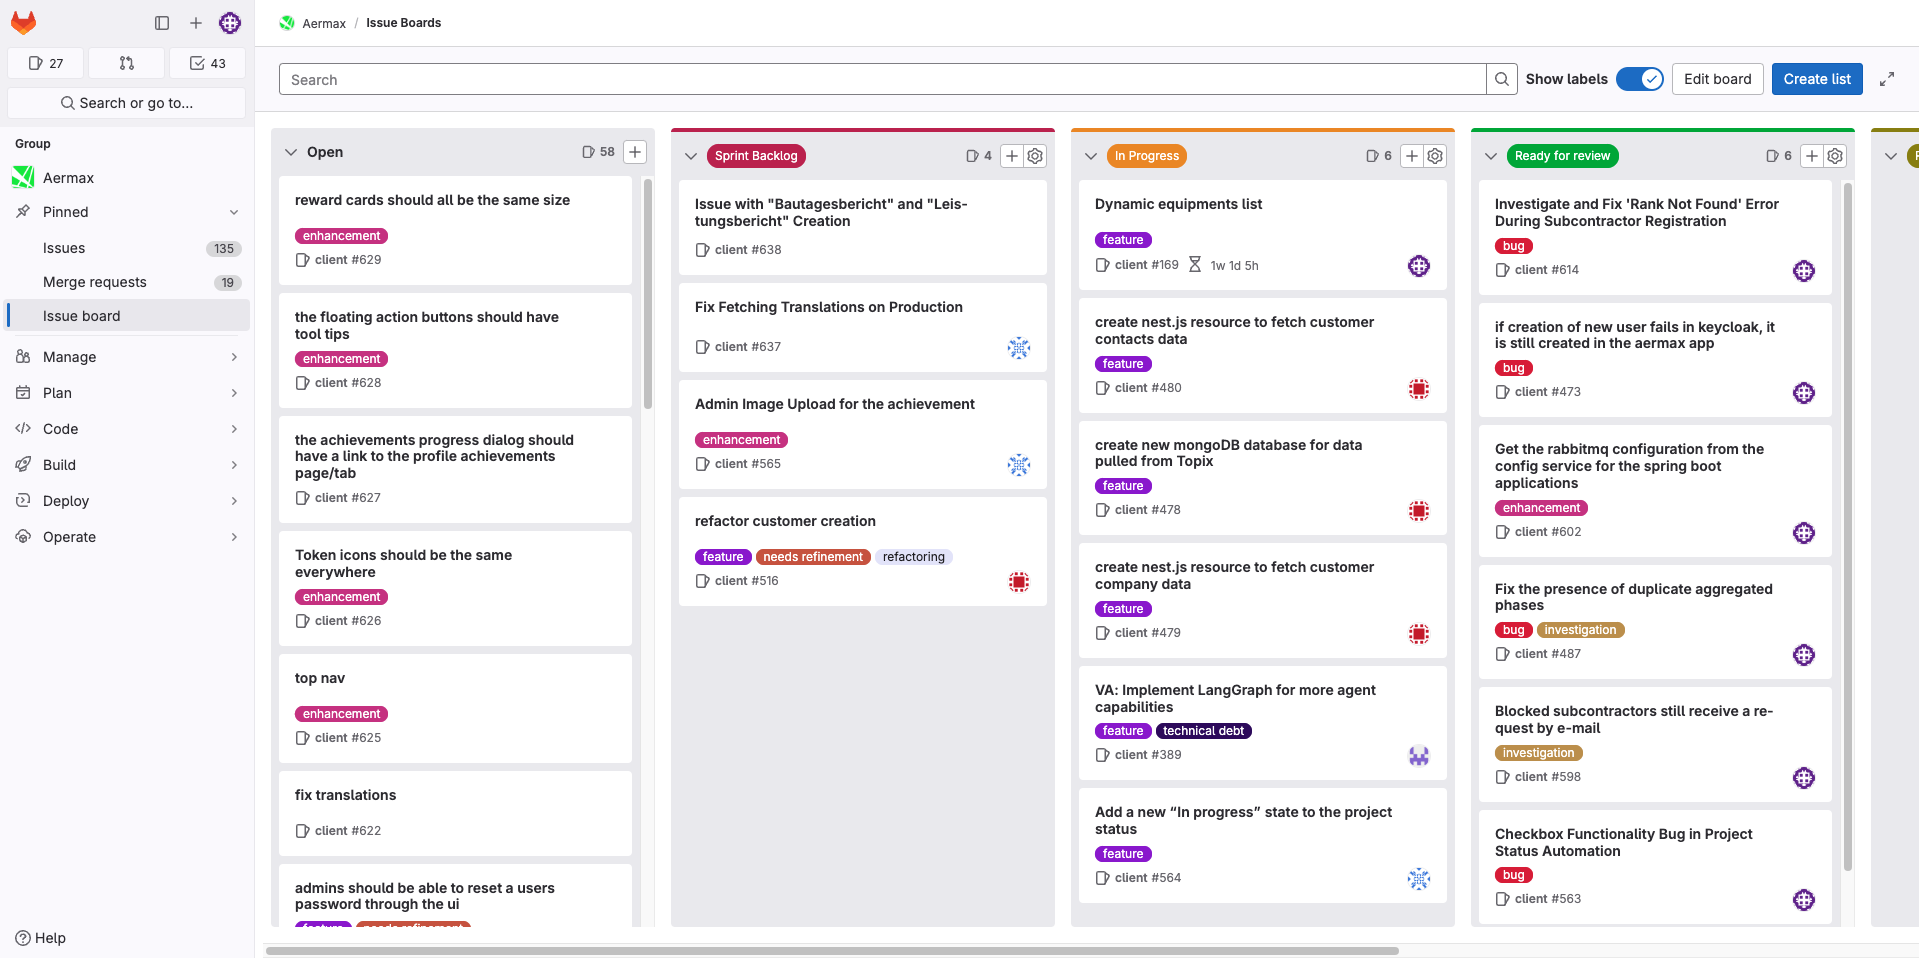
\includegraphics[width=14cm]{src/assets/chapters/aermax-board.png}}
    \caption{Aermax Board}
    \label{fig:armax-board}
\end{figure}
 
\newpage
\subsection{Unified Modeling Language}
The Unified Modeling Language (UML) is a general-purpose, developmental, modeling language in the field of software engineering that is intended to provide a standard way to visualize the design of a system. In our case, we used UML to design the top level view of the systems therefore we only used the Use Case and Sequence diagrams.



\setcounter{secnumdepth}{0} % Set the section counter to 0 so next section is not counted in toc
% ----------------------- Conclusion ----------------------- %
\section{Conclusion}
This chapter introduces the host organization, assesses identified problems and associated challenges, evaluates the competitive landscape, and the adoption of an agile methodology by the team. It also speaks to the next chapter, which is going to deal with the setting of objectives and laying out the roadmap for the remaining sprints under Sprint 0.
